\label{chap:implementation_ground_station }

On the ground station the user only has access to the image viewer program.
The programmer makes use of both the data stream port and the console port to send commands to and receive JPEG photos from the UAV.

\section{The development process} 
Because the GUI includes many functions on the application and links to the TCP/IP ports, the GUI part consider as a very big program. 
Therefore, in order to complete the GUI step by step, a plan for the development is required.
The connection to the datastream can be done by using a console application described in section\ref{sec:testing_connection_send_to_stream}.
When the connection is established, the appliction can listen to the data stream port as in section\ref{sec:testing_receive_stream}.
These console applications will be incorporated into a larger program in later section \ref{completeSystem}. 

These are the development stages that the GUI has went through:

\flushleft
\begin{enumerate}

\item	Understanding what the customer wants. 

\item	Determining the hardware and software specifications.
 
\item	Designing the GUI.

\item  Developing a smaller program which simulates the UAV camera's signals in order to make the testing easier and less time consuming. 

\item	Learning the .NET class that can support the connection to TCP/IP, and communicate between the host and device.

\item	Using GUI to link the ground station software to access the UAV.

\item	Distributing the GUI.
\end{enumerate}

\section{Initial Use Case Diagram}
The use case diagram shows what functions the user can use in the program.
It includes all the specification that the customer wants for a complete system.
Figure~\ref{GUI_useCase} shows all possible actions the user can perform on the program, such as saving, opening and deleting any JPEG image from the computer. 
The user can also connect to the UAV if it is not already connected.
He can use the image viewer program to prompt the UAV payload to return an image which will be displayed on the picture box.
\begin{figure}[H]
\begin{center}
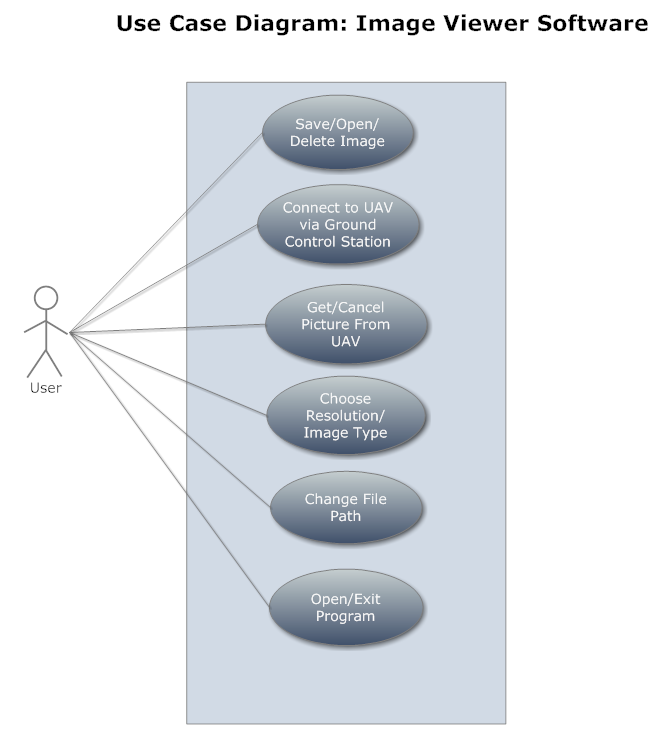
\includegraphics[scale=0.6]{figures/userCase.png} 
\end{center}
\caption{Use case diagram of the GUI\label{GUI_useCase}}
\end{figure}

\begin{figure}[!hbtp]
\begin{center}
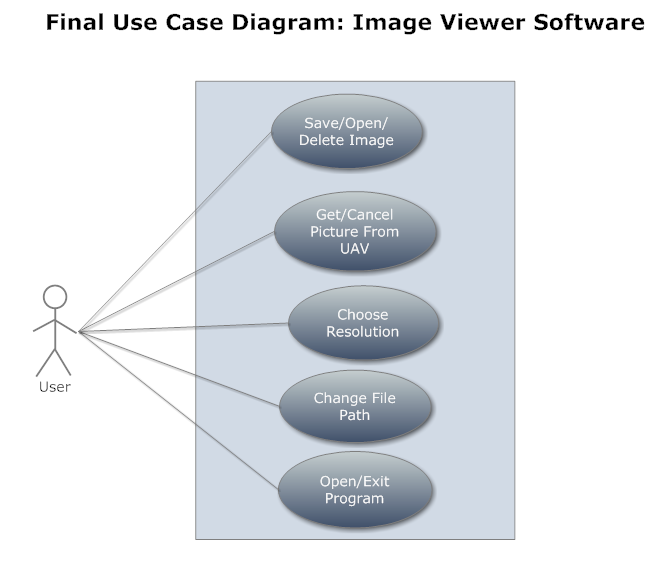
\includegraphics[scale=0.7]{figures/FinaluserCase.png} 
\end{center}
\caption{Final use case diagram of the GUI\label{GUI_finalUseCase}}
\end{figure}

\section{The Design}

The user of our application is assumed to have limited programming experience, so the program will need to be simple to understand. Figure~\ref{ini_GUI} show the first prototype view of the GUI. 
During the downloading process, the application should stay active so that the cancel button can be used. 
The \texttt{Gallery} button will link to another page which will show a gallery of images taken. 
The \texttt{Left} and \texttt{Right} buttons can navigate the picture box to view an earlier picture or a later picture. 
The \texttt{Cancel} button will cancel the download of the receiving image, so that corrupted pictures can be cancel. 
The user mode of the application can access only the main features, such as taking picture, changing directory, and cancelling the download of a picture.  
It allows the user to choose the resolution and picture type (raw or JPEG) to be transmitted from the UAV to the ground station. However, the user doesn't have access to changing the command sent, changing the receiving data, and any interaction with the UAV because to avoid of any errors. 

\begin{figure}[H]
\begin{center}
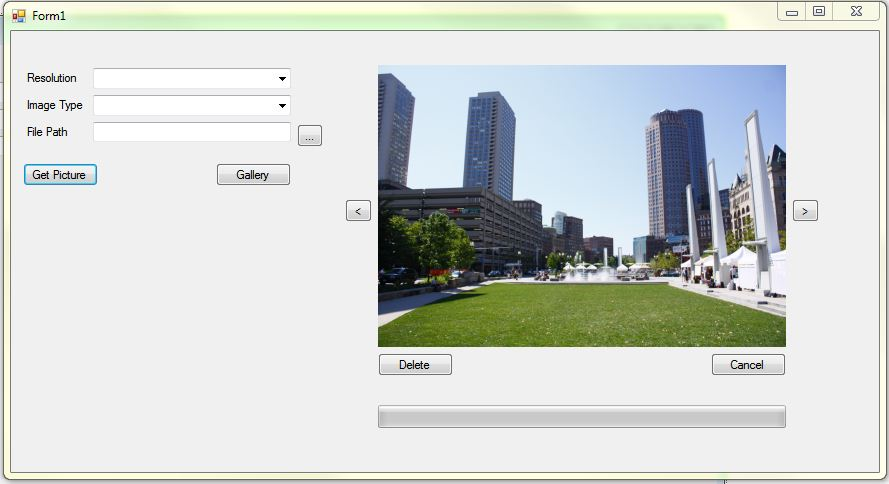
\includegraphics[width=1.0\textwidth]{figures/initialGUI.png} 
\end{center}
\caption{The initial design of GUI\label{ini_GUI}}
\end{figure}
The GUI has been planned to have functions such as auto triggering, selecting the image type, the resolution type, and file path chosen, a progress bar, a help button, and stop and delete buttons. Figure \ref{finalGUI} is the screen shot of the final GUI.

\begin{figure}[H]
\begin{center}
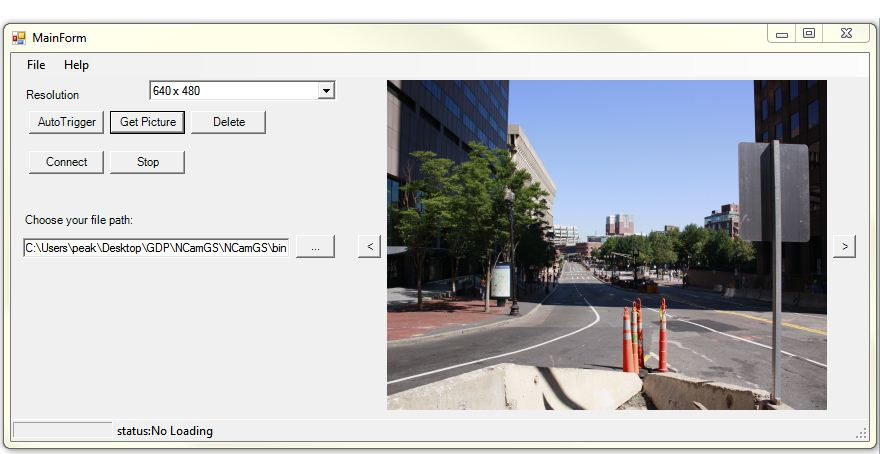
\includegraphics[width=1.0\textwidth]{figures/finalGUI.png} 
\end{center}
\caption{final GUI\label{finalGUI}}
\end{figure}

\section{Final Use Case Diagram}
Figure \ref{GUI_finalUseCase} shows the final use case diagram.
The connect button was not implemented because the ground station will connect automatically to the UAV when the program is opened.
The raw image is too large and takes to long to send down the connection so it was not implemented.
Therefore, the Milestone\ref{sec:ms_pl_img_gs_cam_colour_type} will not be implemented.

\section{Class Diagram}
\subsection*{The Initial Class Diagram}
Figure~\ref{ini_Class} shows initial classes and methods of the image viewer program.
The \texttt{JPEGFileReader} Class has functions for decoding and encoding the JPEG file.
There will be a decoding/encoding algorithm because the image will take a long time to download to the ground station. 

\begin{center}
\begin{figure}[!hbtp]
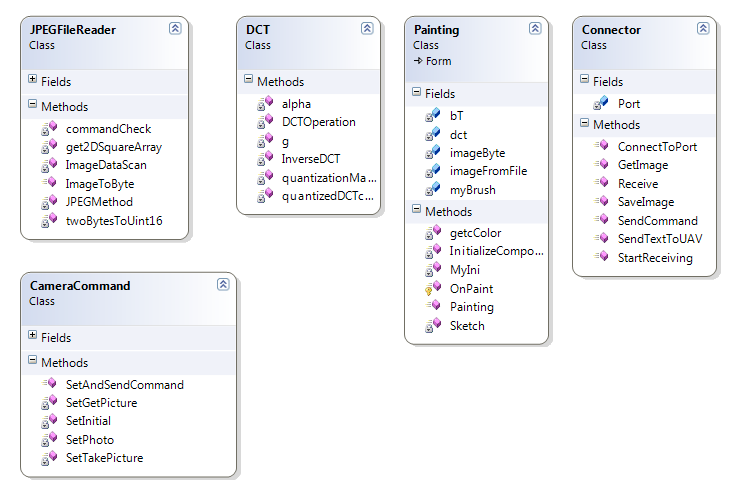
\includegraphics[width=150mm,height=100mm]{figures/initialClassDiagram.png} 
\caption{The initial design of GUI classes\label{ini_Class}}
\end{figure}
\end{center}

The \texttt{DCT} class has many arithmetic operations and equations which have to be implemented on the image viewer program. 

The \texttt{Painting} class is supported by the \texttt{DCT} class. The intention of this class is to display an encoded image point by point on the \texttt{pictureBox}.
Using this method, the \texttt{pictureBox} can display an image from the first pixel transmitted.

The \texttt{CameraCommand} class is designed to send the data from the ground station to the camera. The idea is to make the camera sync with the payload by using ground station commands. The \texttt{SetAndSendCommand} class is used to set the byte command and then send it to the payload via the console port. The \texttt{SetGetPicture()},\texttt{SetInitial()}, \texttt{SetPhoto()}, and \texttt{SetTakePicture()} methods are used for setting the correct byte to send through the \texttt{SetAndSendCommand} class.

\subsection*{The Class Diagram}
The class diagram has been implemented very differently from the planned one.
This is because the new plan is to decode the image on board the UAV and then transmit that image to the ground station in a compressed JPEG file. 
The \texttt{DCT} class is not needed anymore because all the DCT calculation will be done onboard the UAV. 
The \texttt{CameraCommand} has been taken away because the payload will receive an image viewer command from the ground station and then the payload will send another different signal to the camera.
Therefore, the command sent to the camera from the payload does not have to be the same as the command sent from the ground station to the payload. 
The \texttt{Painting} class is used to draw each pixel onto the \texttt{pictureBox}, but it has not been implemented in the final program because the JPEG encoding will be done onboard the UAV.
Therefore, the milestone\ref{sec:ms_pl_img_gs_progressive_dl} will not be implemented.
This is also due to the time limitations.
More detail about the progressive image can be found in the section\ref{sec:implementation_progressive_jpeg}.
 
\begin{figure}[!hbtp]
\begin{center}
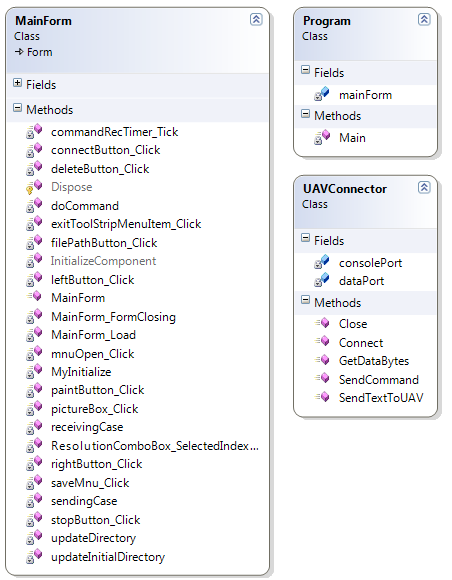
\includegraphics[scale=0.7]{figures/finalClassDiagram.png} 
\end{center}
\caption{Final class diagram of the GUI\label{GUI_finalClassDiagram}}
\end{figure}

\section{Before Connection to the Image Viewer Program}
Figure \ref{schemetic_clipA} shows a diagram of how the connection of the hardware should be. 
The UAV ground receiver is a USB-compatible device that uses Zigbee to communicate. 
The USB device driver has been developed by the customer so the hardware can be accessed by the ground station software, and other applications. 
The USB is active when the host asks for a data. 
A host is the computer network which the UAV connects to. 
The data is in queue until the host asks for the data. 
\begin{figure}[!hbtp]
\begin{center}
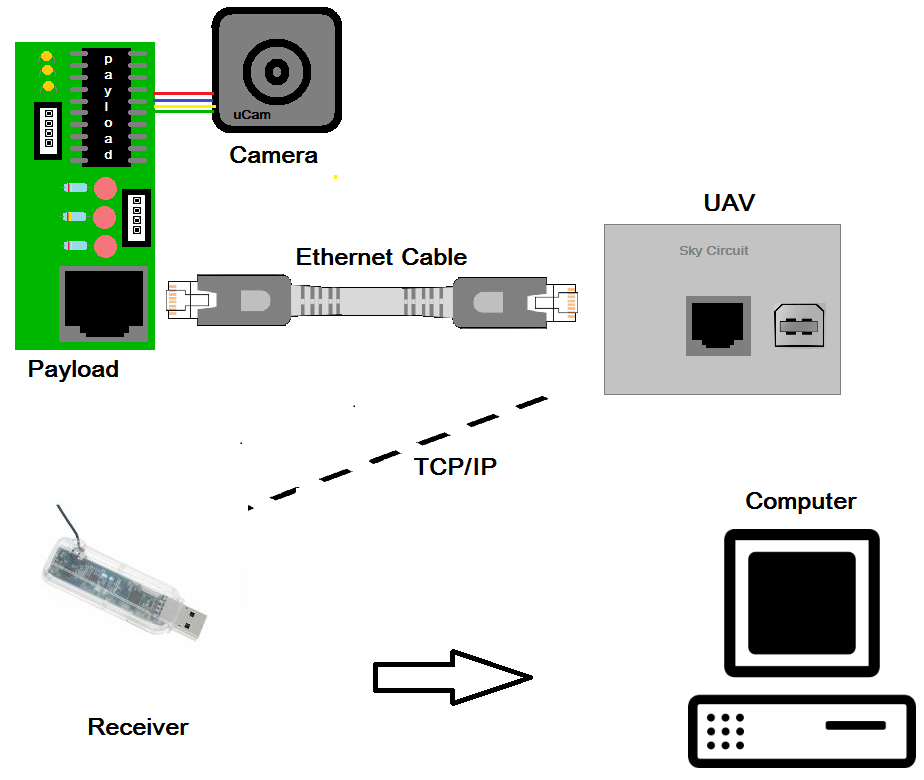
\includegraphics[scale=0.4]{figures/clipArt.png} 
\end{center}
\caption{The connection of the hardware\label{schemetic_clipA}}
\end{figure}


\section{GUI data flow diagram}

Table~\ref{command_table} shows how the command is sent and received to and from the ground station.  Figure~\ref{GCS_Payload_comm} gives a brief detail of how the data communicates between the payload and the image viewer program. 
A more detailed diagram on the data communication can be found in the figure \ref{sequence diagram}.
This has been tested in section\ref{sec:send_console}.

\begin{figure}[H]
\begin{center}
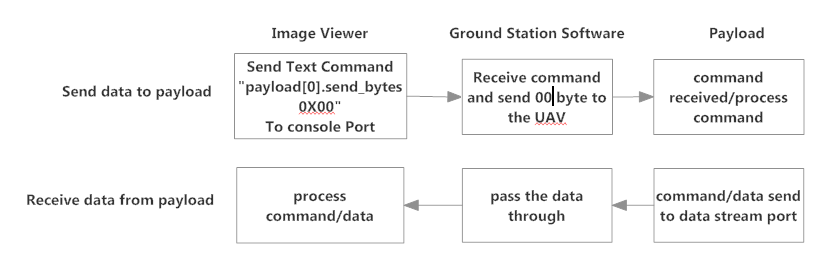
\includegraphics[scale=0.6]{figures/GCS_Payload_communication.png} 
\caption{The connection of data stream port\label{GCS_Payload_comm}}
\end{center}
\end{figure}

\begin{table}[H]

\begin{center}
\begin{tabular}{l l @{.} l}
 Command&
\multicolumn{2}{l}{Address Byte } \\

\hline
\underline{Command from Ground} & \\
SEND\_ZERO\_TOKEN & 0 \\
TAKE\_PICTURE & 0 \\
SEND\_DOWNLOAD\_REQUEST & 2 [MSB] [LSB]  \\
\\
\underline{Command received at Ground}\\
PICTURE\_TAKEN & 1 [MSB] [LSB]\\
DOWNLOAD\_INFO & 3 [MSB] [LSB]\\
IMAGE\_DATA & 4 $\overbrace{ [packet number]}^{2bytes} \overbrace{[image data]}^{data length}$ \\
\end{tabular}
\caption{Command table\label{command_table}}
\end{center}
\end{table}

\section{Get Image Algorithm}
\label{get image algorithm}
When the user clicks on the \texttt{Get Picture} button, the program should send a \textbf{string command} to the ground station software.
Then, the ground station software generates a \textbf{byte command} to be transmitted by TCP to the payload. 
Afterwards, the payload sends a ''Picture Taken'' command back through the data stream port to the Image Viewer Program.

When the program starts running, it initializes the port and commands the customer's application to tell the UAV to stream data to the data stream port. Figure~\ref{GCS_connect_command} shows the connection between the UAV data stream port and the ground station.

\begin{figure}[!hbtp]
\begin{center}
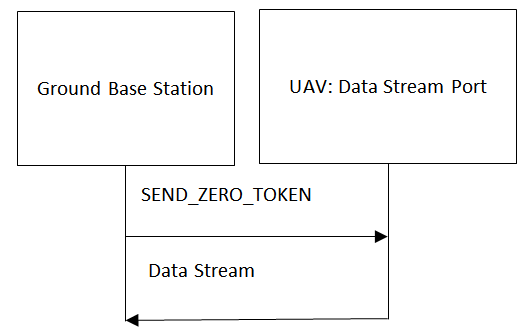
\includegraphics[scale=0.5]{figures/connect_command.png} 
\end{center}
\caption{The connection of data stream port\label{GCS_connect_command}}
\end{figure}

 
\section{Important Code}

This section describes the code that is important for the program. The entire code will not be described but it will be in the appendices. The program must be able to perform these actions to the port: connect to, receive data from and send data to. 

The following .NET C\# classes will be used in the ground station program:
\begin{itemize}
	\item \texttt{FileStream} creates a file. 
	\item \texttt{BinaryWriter} writes the byte data into a specific file made by the \texttt{FileStream} class. 
\end{itemize}

\subsubsection*{UAV Connection}
This section references appendix \ref{appen:UAVConnector} lines 18-38.

The \texttt{Socket} class has functions to send and receive byte and string data. The connection protocol is using the \texttt{PortConnect()} method.  
        
The design of the .NET \texttt{Socket} class simply connects to the port by a \texttt{PortConnect()} command regardless of changes to the baud rate, stop bits, and parity bits. 
This advantage makes the \texttt{Socket} class a more compatible class than the \texttt{SerialPort} class to work with the UAV.
This class has tested using a console application before implementing it in a final GUI. 
This will complete milestone\ref{sec:ms_pl_tx_token_resp}.

\subsection{Start of the program}
This section references appendix \ref{appen:main_form} line 78-87

The \texttt{FileStream} class is initialized by using the method \texttt{FileMode.Create()} in order to generate files. The \texttt{BinaryWriter} writes binary bytes into a file in the directory of the \texttt{FileStream}.
The \texttt{BinaryWriter} class creates a binary file using specific data layout for its bytes. 


\subsection{Text Command}
This section references appendix \ref{appen:UAVConnector} line 68-85.

The TCP/IP protocol transfers data without modifying them. 
It allows the application to freely encode the data \cite{davidB}.
The ground station software allows the Image Viewer program to send a stream composed of a string in bytes. It will then read the command bytes and send it to the payload on the UAV. The codes have shown a correct way to implement the string and send a byte array to the payload.

\texttt{The Socket.Send()} method sends bytes to the ground station software. The ''@ '' sign indicates that the command is correct. For example, consider the bit of code: uavConn.SendTextToUAV(''da 20 payload[0].mem\_ bytes[0]'');
The text \texttt{''da 20 payload[0].mem\_ bytes[0]''} will be converted into a char array and then into a byte array. The byte array will then send the command to the console port and then to the payload through the method \texttt{consolePort.Send(toUAVByte, toUAVChar.Length)}. This will complete Milestone\ref{sec:ms_pl_rx_msg_gs}.

In order to test that the payload receives the same data, we use the oscilloscope to see the signal. The byte displayed on the payload is the same as the byte sent from the ground station. Therefore, the Milestone\ref{sec:ms_pl_img_gs_trigger} is completed. The different resolutions send different byte commands to the payload. The byte commands change if the comboBox options change. Therefore, we can say that Milestone\ref{sec:ms_pl_img_gs_cam_res} has completed.

\begin{lstlisting}[caption={writing binary file},label=lst:writingb]          
	for (int i = 3; i < packetSize; i++)
	{
          opFile.Write(packet[i]);
          numBytes++;
    	}
\end{lstlisting}         

At every cycle of the data being received, the \texttt{opFile.Write()} method will write the packet data into the file in the directory. After the cycle finished, the file will be saved and the image will be displayed in the picture box. 

\subsection{Get Picture Button}
This \texttt{Get Picture} button will use both the send and receive functions of the program. 
The work flow of the \texttt{Get Picture} signal is shown in figure \ref{GUI_finalWorkFlow}.
If the sequence of signal is sent and received correctly, the photo received from the UAV will be displayed on the photo box in the program.
This will complete Milestone\ref{sec:ms_pl_img_sending_gs}.

\begin{figure}[H]
\begin{center}
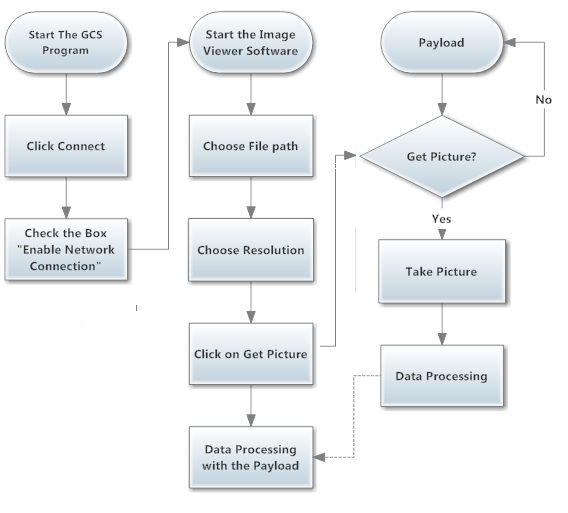
\includegraphics[scale=1]{figures/finalWorkFlow.png} 
\end{center}
\caption{Final work flow diagram of the GUI\label{GUI_finalWorkFlow}}
\end{figure}

\subsection{Implementation - Way-point Triggering (ms)}
\label{sec:waypoint_triggering}

\subsubsection{Description}

The ground station is capable of assigning way-points to
the payload which will allow the camera to take pictures 
at a given location.

This is achieved by sending a simple command script from
the ground station to be uploaded by the payload 
controller. The way-point is designated by the user
through the ground station software. The script 
tells the UAV controller to continuously check the
distance separating itself from the way-point.
When the UAV reaches is within 200 metres of the
way-point, a 0 byte is sent to the camera to prompt
the camera to take a picture.

After taking a picture at the way-point, the camera
is delayed for 10 seconds to avoid taking another picture
at the same way-point. When the 10 second delay is over,
the camera repeats the operation and continuously checks
its distance from the next waypoint.

\subsubsection{Pseudo-code description}

Below is a brief pseudo-code description of the script
sent by the ground station to the payload to take an
image at designated way-points:

\begin{itemize}
	\item while !(UAV distance from next way-point $le$ 200 metres)
		\begin{itemize}
			\item Do nothing.
		\end{itemize}
	\item end while
	\item Prompt camera to take an image.
	\item wait 10 seconds
	\item Re-enter while loop
\end{itemize}

\subsection{Other functions}
The \texttt{Delete} button works like a normal file deleting button. However, when there is only one picture in the file, the program is not allowed to delete that file. This is because even if the pictureBox is set to null, the last image displayed is still pointing to the deleting file. However, the disadvantage of the \texttt{Delete} button is that if the wanted photo was deleted accidentally, it may take a long time to launch the UAV again and take the same photo. 

\begin{figure}[H]
\begin{center}
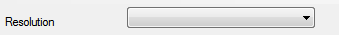
\includegraphics[scale=0.5]{figures/resolutionOption.png} 
\end{center}
\caption{The resolution in combo box\label{resolutionOption}}
\end{figure}

The camera has resolution options as shown in Figure\ref{resolutionOption}. This can be useful when the downloading speed must be fast. The lower the resolution, the faster the data is transmitted to the ground. The GUI's combo box allows the user to choose any wanted resolution in the options. The resolution option gives the user more control over the camera. 

\begin{figure}[H]
\begin{center}
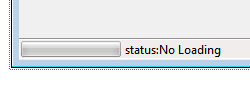
\includegraphics[width=0.3\textwidth]{figures/progressBar.png} 
\end{center}
\caption{The resolution in combo box\label{progressBar}}
\end{figure}

\section{Complete System}
\label{completeSystem}
After implementation has been completed, the different functions will be tested together. When all the parts come together, the ground station program fulfills the requirements of the specification. Figure \ref{completeSystem} shows a final working GUI of our program. 

\begin{figure}[H]
\begin{center}
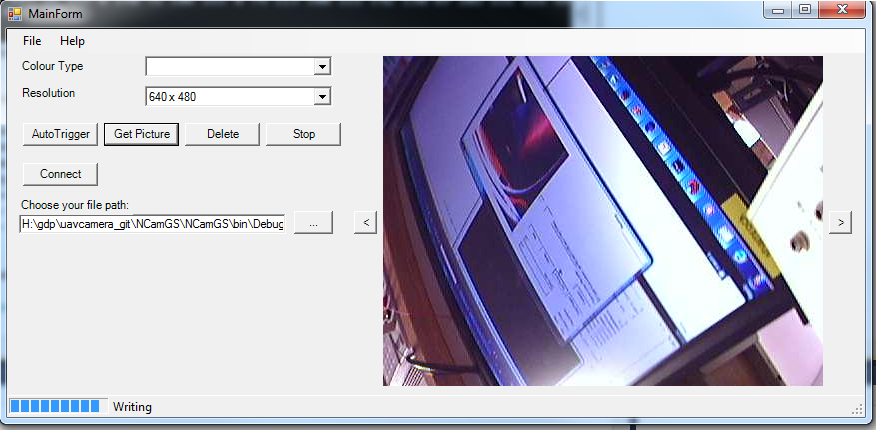
\includegraphics[width=1.0\textwidth]{testing_screenshots/ui.png} 
\end{center}
\caption{The complete system\label{completeSystem}}
\end{figure}


